
% This LaTeX was auto-generated from an M-file by MATLAB.
% To make changes, update the M-file and republish this document.

\documentclass{article}
\usepackage{graphicx}
\usepackage{color}

\sloppy
\definecolor{lightgray}{gray}{0.5}
\setlength{\parindent}{0pt}

\begin{document}

    
    \begin{verbatim}
close all
clear all
rain_long = wavread('./data/rain.wav');
rain_long = mean(rain_long,2);
rain1 = wavread('./data/rain1.wav');
rain1 = mean(rain1,2);
rain2 = wavread('./data/rain2.wav');
rain2 = mean(rain2,2);
rain3 = wavread('./data/rain3.wav');
rain3 = mean(rain3,2);
rain4 = wavread('./data/rain4.wav');
rain4 = mean(rain4,2);
bnoise = wavread('./data/brownnoise.wav');

bckrnd1 = wavread('./data/background1.wav');
bckrnd2 = wavread('./data/background2.wav');

figure
subplot(2,2,1);
plot(abs(fft(rain1)));
title('Rain 1');

subplot(2,2,2);
plot(abs(fft(rain2)));
title('Rain 2');

subplot(2,2,3);
plot(abs(fft(rain3)));
title('Rain 3');

subplot(2,2,4);
plot(abs(fft(rain4)));
title('Rain 4');

figure;
subplot(2,2,1);
spectrogram(rain1);
title('Rain 1');

subplot(2,2,2);
spectrogram(rain2);
title('Rain 2');

subplot(2,2,3);
spectrogram(rain3);
title('Rain 3');

subplot(2,2,4);
spectrogram(rain4);
title('Rain 4');

figure;
subplot(1,2,1);
plot(abs(fft(bckrnd1)));
title('Background1');

subplot(1,2,2);
plot(abs(fft(bckrnd2)));
title('Background2');

figure;
subplot(1,2,1);
spectrogram(bckrnd1);
title('Background1');

subplot(1,2,2);
spectrogram(bckrnd2);
title('Background2');

figure;
subplot(1,2,1);
spectrogram(bnoise);
title('Brown Noise');

subplot(1,2,2);
plot(abs(fft(bnoise)));
title('Brown Noise');
\end{verbatim}

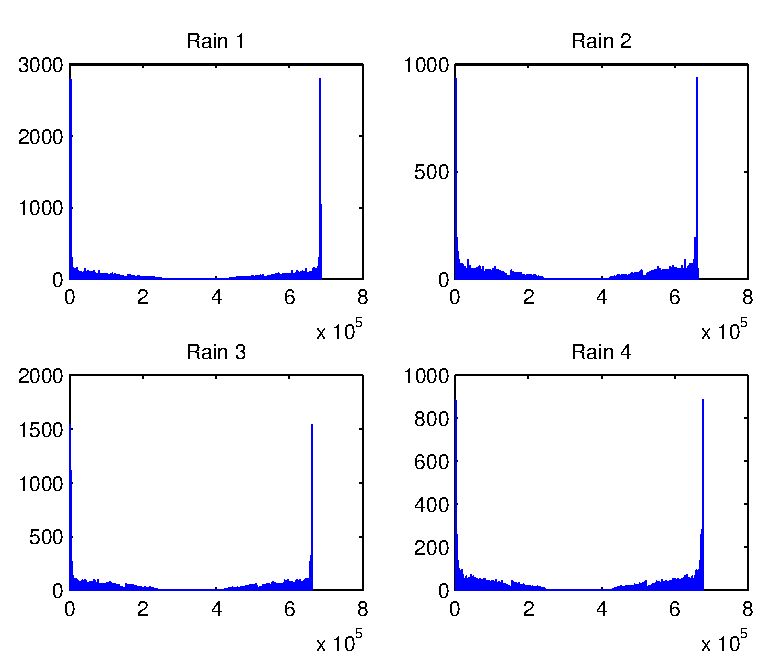
\includegraphics [width=4in]{GetData_01.eps}

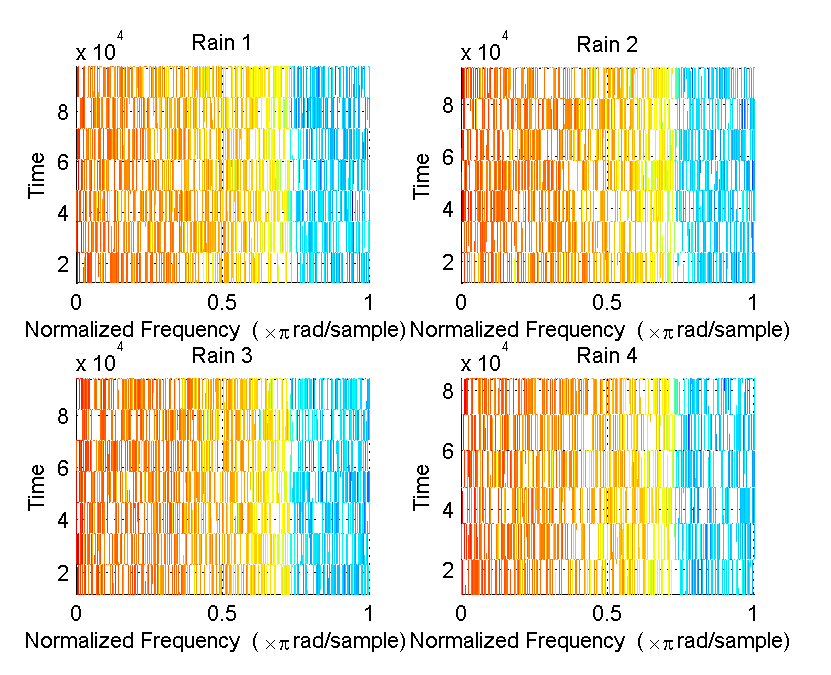
\includegraphics [width=4in]{GetData_02.eps}

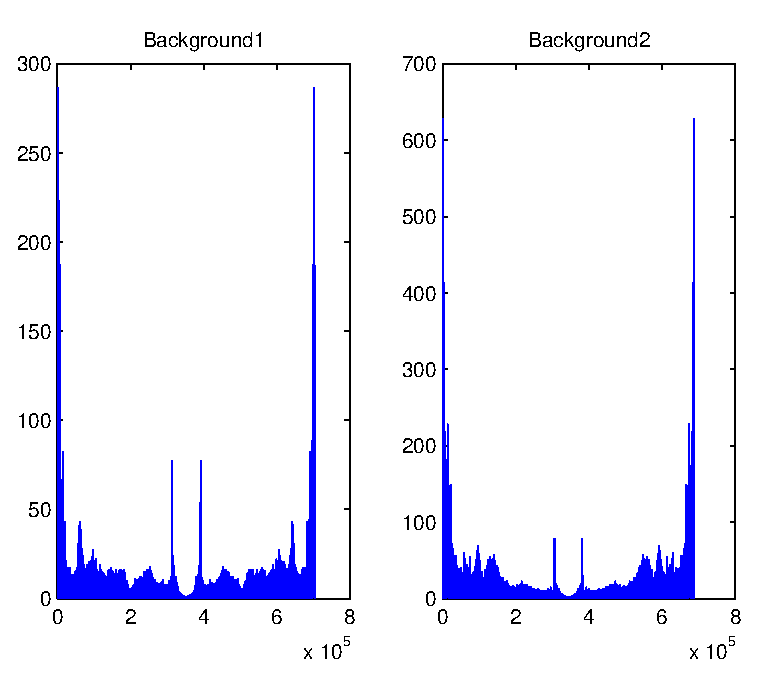
\includegraphics [width=4in]{GetData_03.eps}

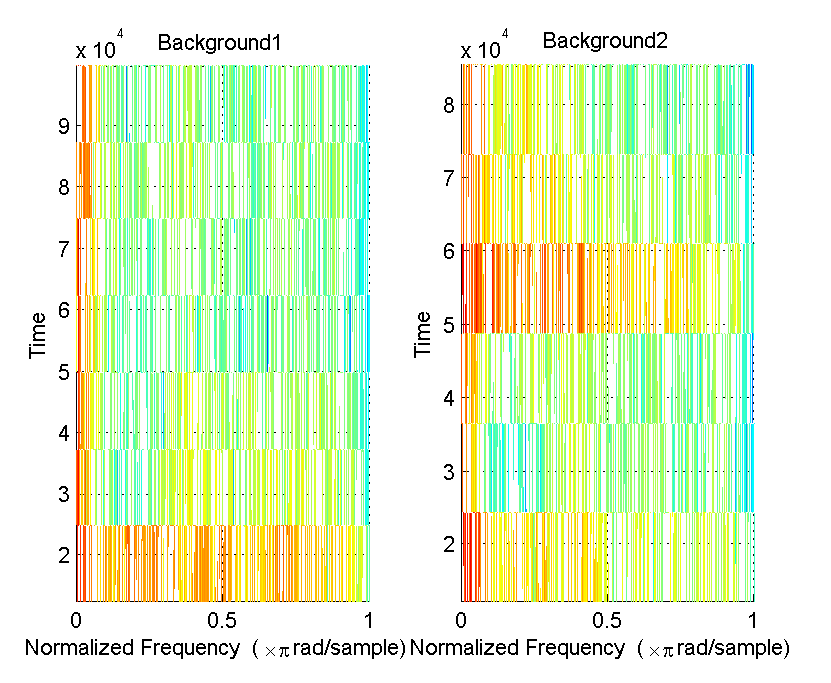
\includegraphics [width=4in]{GetData_04.eps}

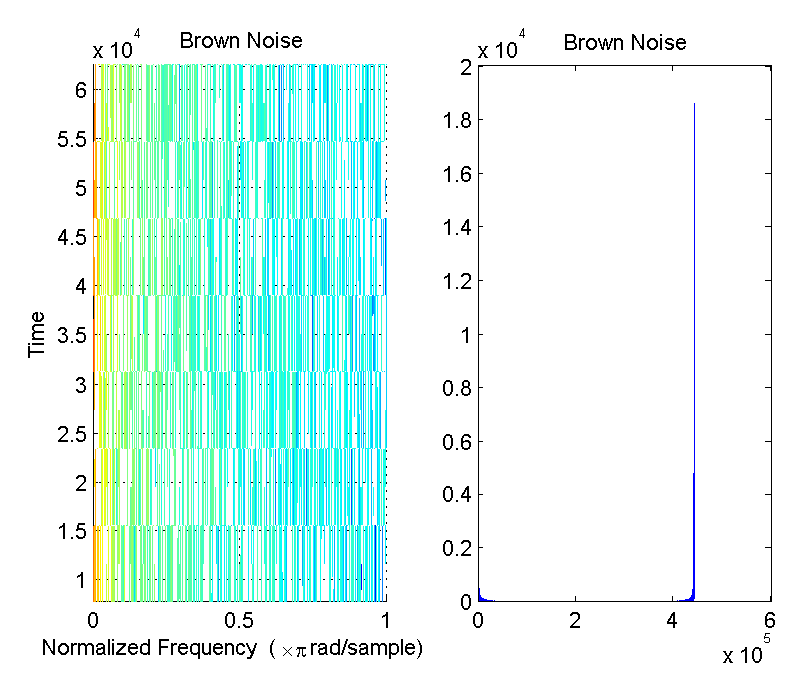
\includegraphics [width=4in]{GetData_05.eps}



\end{document}
    
